\documentclass[a4paper,12pt]{article}
\usepackage{tikz}
\usepackage{amsmath,amssymb,amsthm,enumitem, amsfonts,listings,upquote, graphicx, color}
\usepackage[document]{ragged2e} %left justifies everything automatically
\usepackage{algorithm, algpseudocode}
\usepackage{fancyref}
\usepackage{color} %red, green, blue, yellow, cyan, magenta, black, white
\usepackage{apacite}
\usepackage{geometry}
\usepackage{adjustbox}
% \usepackage{listings}  
\usepackage{graphicx}
\usepackage{float}
\usepackage{tabularx}

\usepackage{listings}
\usepackage{color} %red, green, blue, yellow, cyan, magenta, black, white
\definecolor{mygreen}{RGB}{28,172,0} % color values Red, Green, Blue
\definecolor{mylilas}{RGB}{170,55,241}


\DeclareMathOperator{\prox}{\mathbf{prox}}
\DeclareMathOperator*{\argmin}{arg\,min}

\newcommand{\N}{\mathbb{N}}
\newcommand{\Z}{\mathbb{Z}}

\newcommand\norm[1]{\left\lVert#1\right\rVert}

\lstset{ 
  tabsize=1,
  showstringspaces=false,
  breaklines=true,
}

\addtolength{\oddsidemargin}{-.875in}
\addtolength{\evensidemargin}{-.875in}
\addtolength{\textwidth}{1.75in}
\addtolength{\topmargin}{-.875in}
\addtolength{\textheight}{1.75in}

\definecolor{mygreen}{RGB}{28,172,0} % color values Red, Green, Blue
\definecolor{mylilas}{RGB}{170,55,241}
%%% FIX BELOW
\usepackage{blindtext}
\title{ECS 174 Project 1}
\author{
  Jiayi Lei\\
  SID: 915016668\\
  Email: cjlei@ucdavis.edu
  \and
  Zhengfeng Lai\\
  SID :916678034 \\
  Email: lzhengfeng@ucdavis.edu
} 

%%%\date{SQ 2019}
\date{\today}

\begin{document}
\maketitle

\lstset{language=Matlab,%
    %basicstyle=\color{red},
    breaklines=true,%
    morekeywords={matlab2tikz},
    keywordstyle=\color{blue},%
    morekeywords=[2]{1}, keywordstyle=[2]{\color{black}},
    identifierstyle=\color{black},%
    stringstyle=\color{mylilas},
    commentstyle=\color{mygreen},%
    showstringspaces=false,%without this there will be a symbol in the places where there is a space
    numbers=left,%
    numberstyle={\tiny \color{black}},% size of the numbers
    numbersep=9pt, % this defines how far the numbers are from the text
    emph=[1]{for,end,break},emphstyle=[1]\color{red}, %some words to emphasise
    %emph=[2]{word1,word2}, emphstyle=[2]{style},    
}

\begin{section}{Short Answer Questions}

\begin{subsection}{1}
For clustering points in a continuous vote space, mean-shift would be appropriate. Since it is less time consuming compare to graph-cuts algorithm and easier to run without human supervising compare to k-mean algorithm.
\\

\textbf{1.	K-means algorithm} is an algorithm that tries to cluster points into k groups. The goal of this algorithm is to minimize the sum of distance from points to the center of the group where the points are belonged to. Noticed that we need to put in parameter k into the algorithm, which is sometimes hard to pick. Also, the output will be affected by the initial group centers and the outliers. It needs evaluation of the distance between the hypothesized center to all bins, which is impossible to do with a continuous vote space. 
\\
\textbf{Mean-shift is an algorithm} that moves toward the attraction basin, i.e. the center of the dynamic kernel region.    Compare to k-means algorithm, mean-shift only needs one parameter and can find multiple modes. However, sometimes it is hard to pick the appropriate window size. 
\\
\textbf{Graph-cuts} is an algorithm that tries to minimize the intra distance between points from the same group and maximize the cut value between clusters. The downside of this algorithm is that it is time consuming to run it. It is applied to the situation where the space has been discretized into single units like pixels in an image rather than the case mentioned above.
\\
\end{subsection}


\begin{subsection}{2}

 K-means algorithm, utilizing Euclidian distance as distinguishing criteria, it may have unexpected clustering. If the given dataset is two circles, the results would be two half circles for each cluster rather than two circles by human clustering. And k-means plays poor in clusters within clusters. It attempts to find the center of clusters and then try to minimize the sum of squared differences among all the points near the cluster centers. Therefore, it cannot make the image given, it can only split the circles in half cleanly.

\end{subsection}


\begin{subsection}{3}
\begin{lstlisting}[frame=single]  % Start your code-block



3. First, find the center of mass point for each blob.
Then, extract radius invariant circularity feature.
Finally, cluster the blobs according to their circularity feature.
1) Find the center of mass point for each blob:
for each pixel in blob:
	sum_of_pos += pos(pixel)
	center_of_mass = sum_of_pos/size(blob)
	return center_of_mass
2) Extract radius invariant circularity feature:
radius_mean = size(blob)
for each pixel in boundary(blob):
	sum_square_distance += (center_of_mass-position(pixel))^2
	circularity = sum_square_distance/size(boundry(blob))
	return circularity
3) Clusters k-means(circularity[],k)
	return k-means = circularity[]

\end{lstlisting}
\end{subsection}

\end{section}


\begin{section}{Short Programming}
\begin{subsection}{(a)}
Matlab CODE:\\
\begin{lstlisting}[frame=single]  % Start your code-block
%% (a)
clc;clf;clear all;
inputIm = imread('wdc1.jpg');
refIm = imread('wdc2.jpg');
points1 = GetPoints(inputIm);
points2 = GetPoints(refIm);
save points.mat points1 points2 

\end{lstlisting}


\end{subsection}

\begin{subsection}{(b)}
\textbf{computedH.m} is attached in the folder we submitted and also the code is attatched in the appendix section for your convenience to read.  


\end{subsection}

\begin{subsection}{(c)}
\textbf{warpImage.m} is attached in the folder we submitted and also the code is attatched in the appendix section for your convenience to read.  


\end{subsection}

\clearpage
\begin{subsection}{(d)}

\textbf{points.mat} is attatched in the folder.
\\
\textbf{Output for crop1.jpg and crop2.jpg}\\

 \begin{figure}[!htb]
       \center
       {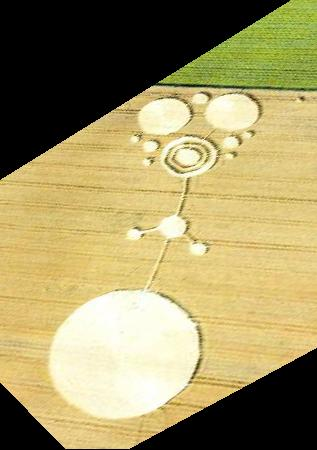
\includegraphics[width=10cm]
       {crop_warp.png}}
        \caption{Warped Image of crop 1}
      \end{figure}



\begin{figure}[!htb]
        \center{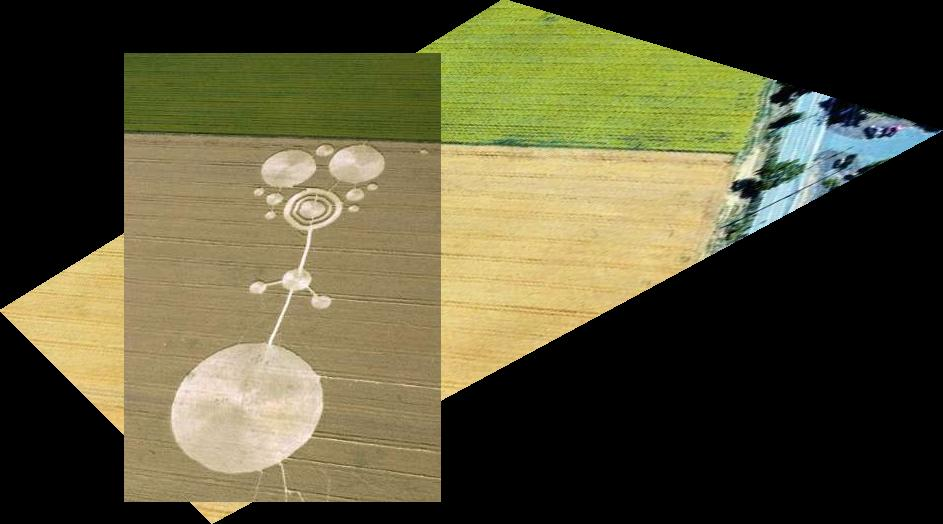
\includegraphics[width=10cm]
        {crop_merge.png}}
        \caption{Merge Image of crop1 and crop2}
      \end{figure}
      
      
      
\textbf{Output for wdc1.jpg and wdc2.jpg}\\

 \begin{figure}[!htb]
       \center
       {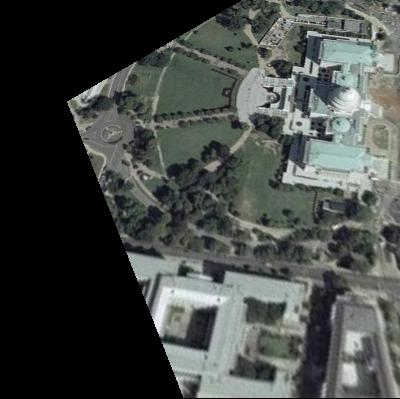
\includegraphics[width=10cm]
       {wdc_warp.png}}
        \caption{Warped Image of wdc1}
      \end{figure}



\begin{figure}[!htb]
        \center{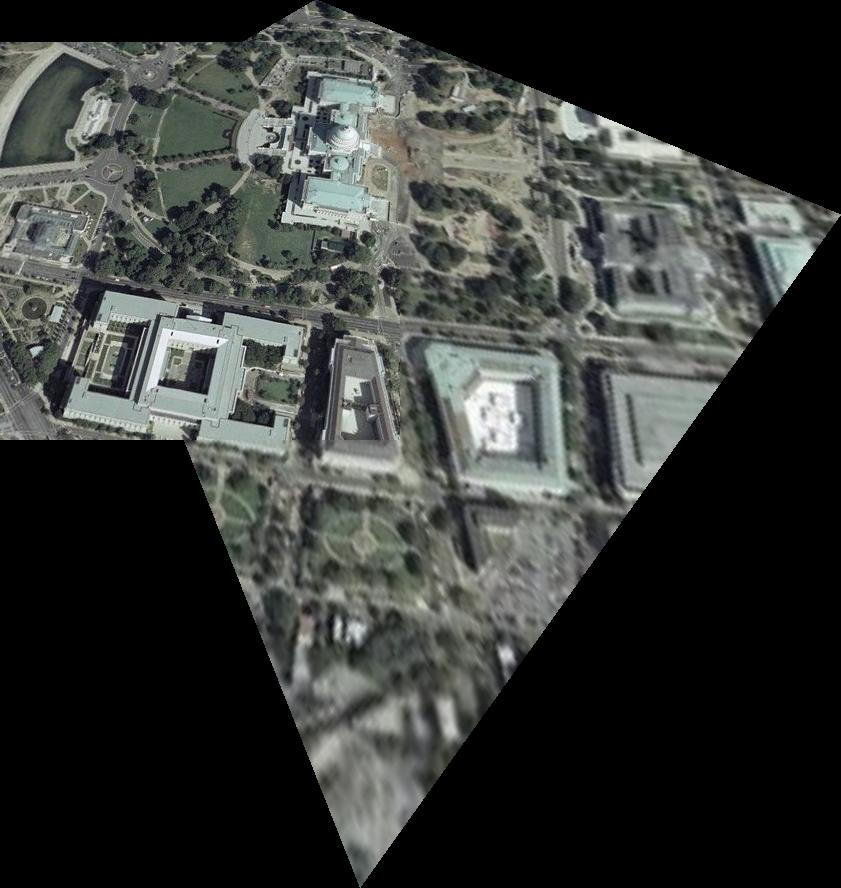
\includegraphics[width=10cm]
        {wdc_merge.png}}
        \caption{Merge Image of wdc1 and wdc2}
      \end{figure}
      

\end{subsection}

\clearpage
\begin{subsection}{(e)}
\textbf{Another Example with MU1 and MU2}\\

 \begin{figure}[!htb]
       \center
       {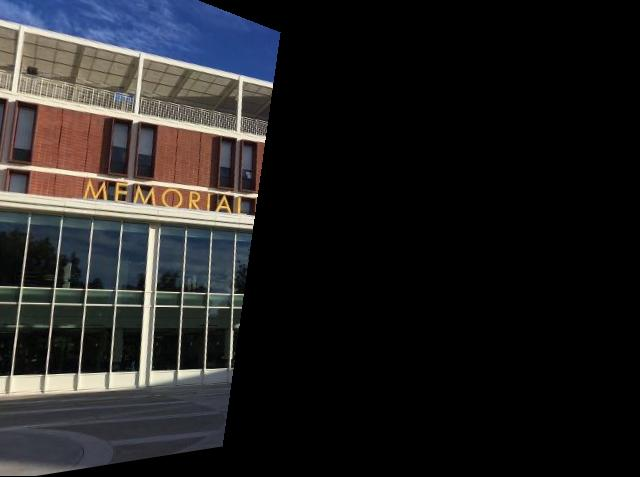
\includegraphics[width=10cm]
       {MU_warp.png}}
        \caption{Warped Image of MU1}
      \end{figure}



\begin{figure}[!htb]
        \center{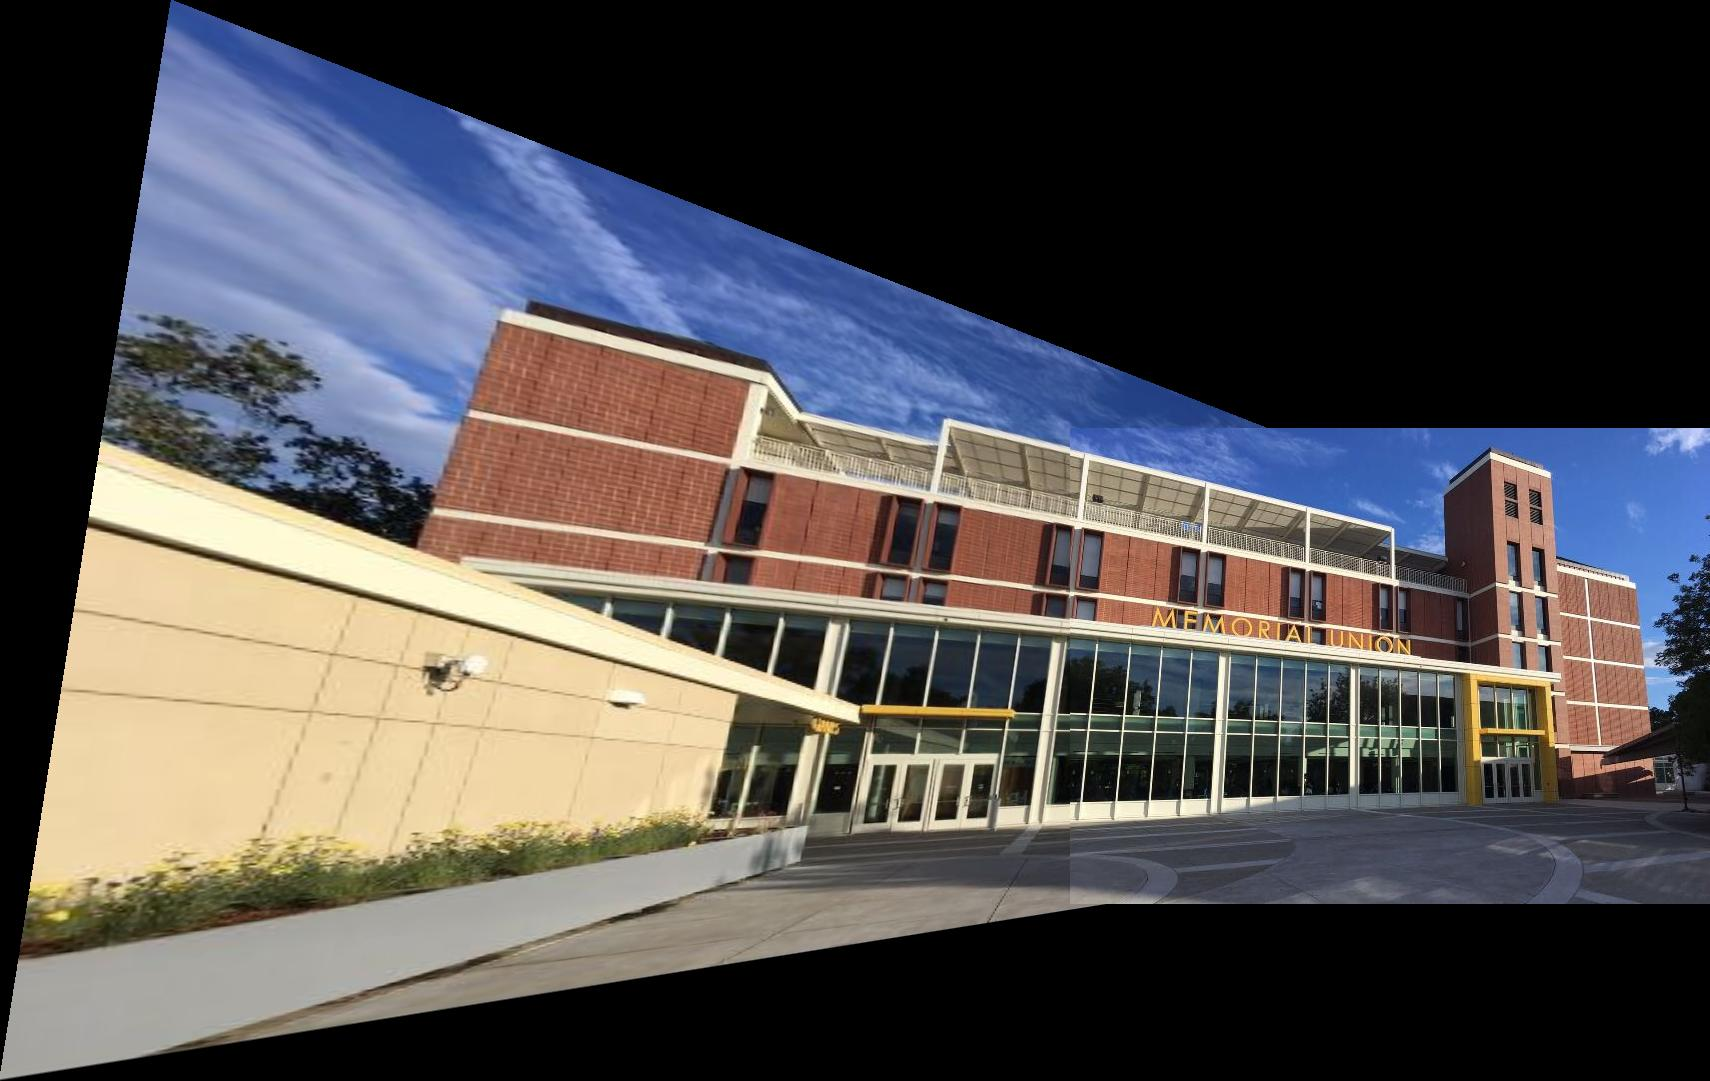
\includegraphics[width=10cm]
        {MU_merge.png}}
        \caption{Merge Image of MU1 and MU2}
      \end{figure}
      


\end{subsection}
\clearpage
\begin{subsection}{(f)}


\end{subsection}

\end{section}

\clearpage
\begin{section}{Extra Credit}
\begin{lstlisting}[frame=single]  % Start your code-block
%% Optional (a) RANSAC
clc;clf;
inputIm = imread('crop1.jpg');
refIm = imread('crop2.jpg');
t1 = importdata('cc1.mat');
t2 = importdata('cc2.mat');
H = RANSAC(t1,t2);
disp(H);
[warpIm, mergeIm] = warpImage(inputIm, refIm, H);
imwrite(warpIm,'crop_warp_RANSAC.jpg');
imwrite(mergeIm,'crop_merge_RANSAC.jpg');

\end{lstlisting}

\textbf{OUTPUTS:}
\\

 \begin{figure}[!htb]
       \center
       {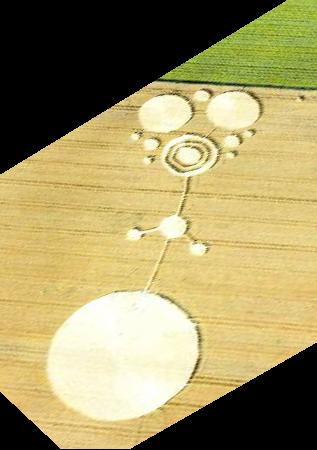
\includegraphics[width=10cm]
       {crop_warp_RANSAC.png}}
        \caption{Warped Image by using RANSAC}
      \end{figure}



\begin{figure}[!htb]
        \center{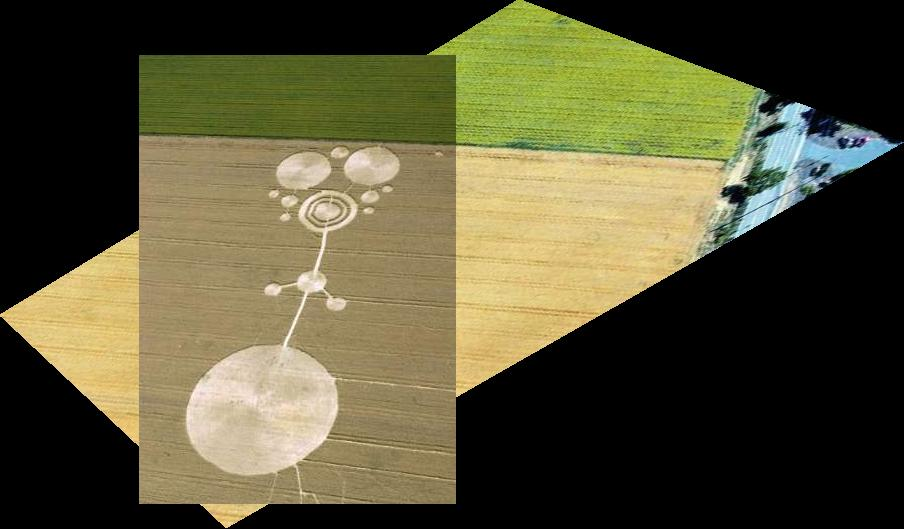
\includegraphics[width=10cm]
        {crop_merge_RANSAC.png}}
        \caption{Merge Image oby using RANSAC}
      \end{figure}

\end{section}


\clearpage
\begin{section}{Appendix}
\begin{subsection}{computeH.m}
\section*{Matlab Code}

\lstinputlisting{computeH.m}

\end{subsection}


\clearpage

% warpImage.m


\begin{subsection}{warpImage.m}
\section*{Matlab Code}

\lstinputlisting{warpImage.m}

\end{subsection}

\end{section}

\end{document}